\documentclass[a4paper]{article}
\usepackage[utf8]{vntex}
\usepackage{wrapfig}
%\usepackage[english,vietnam]{babel}
%\usepackage[utf8]{inputenc}
\usepackage{mathptmx}[ptm]
%\usepackage[utf8]{inputenc}
%\usepackage[francais]{babel}
\usepackage{a4wide,amssymb,epsfig,latexsym,array,hhline,fancyhdr}
\usepackage[normalem]{ulem}
%\usepackage{soul}

\usepackage[makeroom]{cancel}
\usepackage{amsmath}
\usepackage{amsthm}
\usepackage{multicol,longtable,amscd}
\usepackage{diagbox}%Make diagonal lines in tables
\usepackage{booktabs}
\usepackage{alltt}
\usepackage[framemethod=tikz]{mdframed}% For highlighting paragraph backgrounds
\usepackage{caption,subcaption}

\usepackage{lastpage}
\usepackage[lined,boxed,commentsnumbered]{algorithm2e}
\usepackage{enumerate}
\usepackage{color}
\usepackage{graphicx}							% Standard graphics package
\graphicspath{{images/}{Images/}}
\usepackage{array}
\usepackage{tabularx, caption}
\usepackage{multirow}
\usepackage{multicol}
\usepackage{rotating}
\usepackage{graphics}
\usepackage{geometry}
\usepackage{setspace}
\usepackage{titlesec}
\usepackage{indentfirst}
\usepackage{epsfig}
\usepackage{tikz}
\usepackage{eso-pic}

\usetikzlibrary{arrows,decorations.pathmorphing,backgrounds,calc,positioning,shapes.geometric}

% Cover frame in absolute paper coordinates so it cannot drift
\newcommand{\InternshipCoverFrame}{%
  \AddToShipoutPictureBG*{%
    \AtPageLowerLeft{%
      
\begin{tikzpicture}
        \useasboundingbox (0,0) rectangle (\paperwidth,\paperheight);
        \draw[line width=4pt]
          (0.40in,0.50in) rectangle (\paperwidth-0.40in,\paperheight-0.50in);
        \draw[line width=1.5pt]
          (0.45in,0.55in) rectangle (\paperwidth-0.45in,\paperheight-0.55in);
      \end{tikzpicture}%
    }%
  }%
}

\usepackage[unicode]{hyperref}
\hypersetup{urlcolor=blue,linkcolor=black,citecolor=black,colorlinks=true} 
\usepackage{listings}

%\usepackage{pstcol} 								% PSTricks with the standard color package

\usepackage[normalem]{ulem}

\newtheorem{theorem}{{\bf Định lý}}
\newtheorem{property}{{\bf Tính chất}}
\newtheorem{proposition}{{\bf Mệnh đề}}
\newtheorem{corollary}[proposition]{{\bf Hệ quả}}
\newtheorem{lemma}[proposition]{{\bf Bổ đề}}
\theoremstyle{definition}
\newtheorem{exer}{Bài toán}

\def\thesislayout{	% A4: 210 × 297
	\geometry{
		a4paper,
		total={160mm,240mm},  % fix over page
		left=30mm,
		top=30mm,
	}
}
\def\thesisheadlayout{	% A4: 210 × 297
	\geometry{
		a4paper,
		total={160mm,240mm},  % fix over page
		left=30mm,
		top=10mm,
	}
}
\thesislayout
\lstset{
language=R,
basicstyle=\footnotesize\sffamily,
commentstyle=\ttfamily\color{black},
numbers=left,
numberstyle=\ttfamily\color{black}\footnotesize,
stepnumber=1,
numbersep=5pt,
backgroundcolor=\color{white},
showspaces=false,
showstringspaces=false,
showtabs=false,
frame=single,
tabsize=2,
captionpos=b,
breaklines=true,
breakatwhitespace=false,
title=\lstname,
escapeinside={},
keywordstyle={},
morekeywords={}
}
%\usepackage{fancyhdr}
\setlength{\headheight}{40pt}
\pagestyle{fancy}
\fancyhead{} % clear all header fields
\fancyhead[L]{
 \begin{tabular}{rl}
    \begin{picture}(25,15)(0,0)
    \put(0,-8){
\includegraphics[width=10mm, height=10mm]{hcmut.png}}
    %\put(0,-8){\epsfig{width=10mm,figure=hcmut.eps}}
   \end{picture}&
	%
\includegraphics[width=8mm, height=8mm]{hcmut.png} & %
	\begin{tabular}{l}
		\textbf{  Trường Đại Học Bách Khoa - Đại học Quốc gia TP.HCM }\\
		\textbf{  Khoa Điện - Điện Tử}
	\end{tabular} 	
 \end{tabular}
}
\fancyhead[R]{
	\begin{tabular}{l}
		\tiny \bf \\
		\tiny \bf 
	\end{tabular}  }
\fancyfoot{} % clear all footer fields
\fancyfoot[L]{\scriptsize  Báo cáo môn học (EE3067) - HK1 2026- 2027}
\fancyfoot[R]{\scriptsize  Trang {\thepage}/\pageref{LastPage}}
\renewcommand{\headrulewidth}{0.3pt}
\renewcommand{\footrulewidth}{0.3pt}


%%%
\setcounter{secnumdepth}{4}
\setcounter{tocdepth}{3}
\makeatletter
\newcounter {subsubsubsection}[subsubsection]
\renewcommand\thesubsubsubsection{\thesubsubsection .\@alph\c@subsubsubsection}
\newcommand\subsubsubsection{\@startsection{subsubsubsection}{4}{\z@}%
                                     {-3.25ex\@plus -1ex \@minus -.2ex}%
                                     {1.5ex \@plus .2ex}%
                                     {\normalfont\normalsize\bfseries}}
\newcommand*\l@subsubsubsection{\@dottedtocline{3}{10.0em}{4.1em}}
\newcommand*{\subsubsubsectionmark}[1]{}
\makeatother

\everymath{\color{black}}%make in-line maths symbols blue to read/check easily

% --- Thiết lập dàn trang và dãn dòng ---
% Dãn dòng vừa phải, phù hợp với báo cáo tiếng Việt.
\setstretch{1.15}
\raggedbottom
\setlength{\parindent}{1.25em}
\setlength{\parskip}{0.35em plus 0.08em minus 0.04em}
\setlength{\emergencystretch}{2em}

% Khoảng cách tiêu đề nhất quán, tránh tiêu đề bị dính vào đoạn văn.
\titleformat{\section}
  {\normalfont\Large\bfseries}
  {\thesection}{0.75em}{}
\titlespacing*{\section}{0pt}{2.2ex plus 0.6ex minus 0.2ex}{1.1ex plus 0.2ex}

\titleformat{\subsection}
  {\normalfont\large\bfseries}
  {\thesubsection}{0.75em}{}
\titlespacing*{\subsection}{0pt}{1.8ex plus 0.5ex minus 0.2ex}{0.8ex plus 0.2ex}

\titleformat{\subsubsection}
  {\normalfont\normalsize\bfseries}
  {\thesubsubsection}{0.75em}{}
\titlespacing*{\subsubsection}{0pt}{1.4ex plus 0.4ex minus 0.2ex}{0.5ex plus 0.1ex}

% Khoảng cách hình, bảng và chú thích cân đối hơn.
\captionsetup[figure]{labelfont={small,bf},textfont={small,it},skip=5pt}
\captionsetup[table]{labelfont={small,bf},textfont={small,it},skip=5pt}
\setlength{\floatsep}{10pt plus 2pt minus 2pt}
\setlength{\textfloatsep}{12pt plus 2pt minus 3pt}
\setlength{\intextsep}{10pt plus 2pt minus 2pt}

\thesislayout

\begin{document}

\hypersetup{pageanchor=false}
\begin{titlepage}
\InternshipCoverFrame

\begin{center}
\Large \textbf{ĐẠI HỌC QUỐC GIA THÀNH PHỐ HỒ CHÍ MINH} \\
\vspace{0.2cm}
\Large \textbf{TRƯỜNG ĐẠI HỌC BÁCH KHOA} \\
\vspace{0.2cm}
\Large \textbf{KHOA ĐIỆN - ĐIỆN TỬ}
\end{center}

\vspace{0.15cm}
\begin{center}

\includegraphics[width=5cm]{hcmut.png}
\end{center}

\vfill
\begin{center}{\Large \textbf{MÔN HỌC}}\end{center}

\begin{center}{\Large TRÍ TUỆ NHÂN TẠO TRONG ĐIỀU KHIỂN}\end{center}
\vfill
\begin{center}{\Large \textbf{"THUẬT TOÁN PLA - PERCEPTION LEARNING ALGORITHM"}}\end{center}
\vfill
\begin{center}{\Large REPORT HOMEWORK 1}\end{center}
\vfill
\begin{center}{\Large Lớp: L01 \quad Nhóm: 05 \quad HK261}\end{center}
\begin{center}{\Large \textbf{GVHD:} TS. PHẠM VIỆT CƯỜNG}\end{center}
\vfill
\begin{center}
\renewcommand{\arraystretch}{1.35}
\begin{tabular}{|c|p{6.4cm}|c|c|}
\hline
\textbf{STT} & \textbf{Sinh viên} & \textbf{MSSV} & \textbf{Điểm} \\
\hline
1 & Nguyễn Văn Tuấn Anh & 2310131 & \\
\hline
2 & & & \\
\hline
3 & & & \\
\hline
4 & & & \\
\hline
\end{tabular}
\end{center}
\vfill
\begin{center}
{\Large TP. Hồ Chí Minh, ngày 23 tháng 09 năm 2026}
\end{center}
\end{titlepage}
\hypersetup{pageanchor=true}
\pagenumbering{arabic}

\tableofcontents

\listoffigures


\newpage
\section{Tóm tắt lý thuyết}
Chương này trình bày bài toán phân lớp nhị phân và thuật toán học Perceptron (Perceptron Learning Algorithm, PLA). 
\subsection{Phân lớp nhị phân}
Bài toán phân lớp nhị phân là phân loại 2 lớp dữ liệu riêng biệt 
(hay còn gọi là binary classification). 

Giả sử có hai class tương ứng hai tập điểm xanh và đỏ,
bài toán đặt ra là từ dữ liệu đã gắn nhãn xanh-đỏ (cho rằng tập 2 dữ liệu này linearly separable), 
ta cần tìm một bộ phân lớp (classifier) có khả năng dự đoán màu của một điểm dữ liệu mới.

\begin{figure}[h]
    \centering
    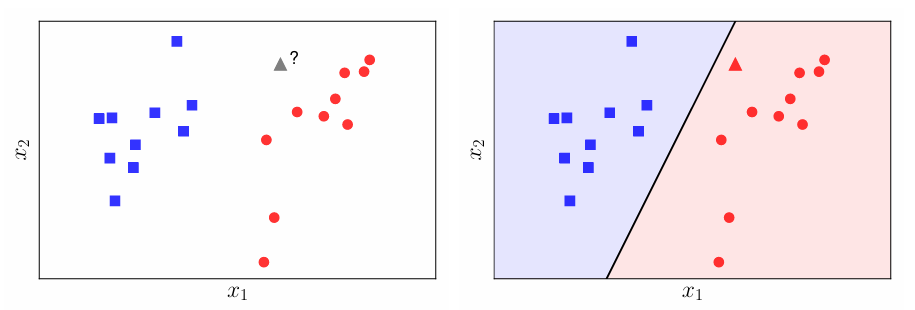
\includegraphics[width=0.5\textwidth]{../images/two-class.png}
    \caption{Bài toán phân lớp nhị phân trong 2D}
\end{figure}

Nếu coi mỗi vector đặc trưng là một điểm trong không gian \(d\) chiều, 
bài toán phân lớp coi như bài toán xác định điểm đó thuộc lớp nào. 
Hay nói cách khác, nếu mỗi lớp chiếm một vùng trong không gian, ta cần xác định
ranh giới (boiundary) giữa các vùng này.

\subsection{Thuật toán perceptron}
\subsubsection{Cách phân lớp}
- Giả sử \(X = [x_1, x_2, \ldots, x_n] \in \mathbb{R}^{d \times N}\) là ma trận vector chứa các điểm huấn luyện.

- \(x_i\) là vector đặc trưng thứ \(i\)

- Nhãn \(y = [y_1, y_2, \ldots, y_n] \in \mathbb{R}^{1 \times N}\)
với \(y_i = 1\) nếu \(x_i\) thuộc lớp 1, \(y_i = -1\) nếu \(x_i\) thuộc lớp 2

Tại một thời điểm, giả sử có boundary là siêu phẳng có pt:
\[
f(\mathbf{x}) = w_1x_1 + \cdots + w_dx_d + w_0
= \mathbf{w}^{T}\mathbf{x} + w_0 = 0
\]

- Với \(\mathbf{w} \in \mathbb{R}^{d}\) là vector hệ số, \(w_0\) là bias (tự do).

- Dùng \textbf{bias trick} để đưa \(w_0\) vào \(\mathbf{w}\), ta có siêu phẳng là

\[
\tilde{\mathbf{x}} = \begin{bmatrix} \mathbf{x} \\ 1 \end{bmatrix}, \qquad
\tilde{\mathbf{w}} = \begin{bmatrix} \mathbf{w} \\ w_0 \end{bmatrix}, \qquad
f(\tilde{\mathbf{x}}) = \tilde{\mathbf{w}}^{T}\tilde{\mathbf{x}} = 0
\]

- Nếu w là nghiệm của bài toán perceptron, với data mới x chưa gán nhãn
, ta có thể gán nhãn bằng cách:
\[
\operatorname{label}(\mathbf{x}) =
\begin{cases}
1 & \text{nếu } \mathbf{w}^{T}\mathbf{x} \ge 0,\\
-1 & \text{o.w.}
\end{cases}
\]

- Nói cách khác, $\operatorname{label}(\mathbf{x}) =
\operatorname{sgn}(\mathbf{w}^{T}\mathbf{x})$ với $\operatorname{sgn}$ là hàm xác định dấu,
giả sử rằng $\operatorname{sgn}(0)=1$.

\subsubsection{Thuật toán phân lớp Perceptron}
Bằng việc xây dựng hàm mất mát:
\[
J(\mathbf{w}) = \sum_{\mathbf{x}_i \in \mathcal{M}}
\left(-y_i \mathbf{w}^{T}\mathbf{x}_i\right)
\]

Trong đó \(\mathcal{M}\) là tập các điểm dữ liệu bị phân lớp lỗi, tức là các điểm dữ liệu mà \(\operatorname{label}(\mathbf{x}_i) \neq y_i\).

Và với một điểm dữ liệu \(x_i\) bị phân lớp lỗi, hàm mất mát và đạo hàm của nó:
\[
J(\mathbf{w}; \mathbf{x}_i, y_i)
= -y_i\mathbf{w}^{T}\mathbf{x}_i,
\qquad
\nabla_{\mathbf{w}}J(\mathbf{w}; \mathbf{x}_i, y_i)
= -y_i\mathbf{x}_i
\]

Và tối ưu hàm mất mát bằng Schoolastic Gradient Descent (SGD):
\[
\mathbf{w} \leftarrow \mathbf{w}
-\eta\left(-y_i\mathbf{x}_i\right)
= \mathbf{w}+\eta y_i\mathbf{x}_i
\]
\section{Giải thích mã nguồn}
Chương này đi theo \textsf{src/basic.py}. Tệp gồm năm khối, đúng với các mục comment trong mã: sinh dữ liệu, các hàm của PLA, chạy thuật toán, vẽ đường phân tách, và hoạt họa từng lần cập nhật. Mỗi mục dưới đây trích đúng khối tương ứng rồi giải thích khối đó làm gì.

\subsection{Khối 1: Sinh hai lớp điểm}
Ba dòng đầu nhập NumPy để tính trên mảng, Matplotlib để vẽ, và \textsf{FuncAnimation} để xuất từng khung hình. Phần sinh dữ liệu là Listing~\ref{lst:data}. Số dòng in bên cạnh mã trùng với số dòng trong \textsf{src/basic.py}.

\lstinputlisting[
  language=Python,
  firstline=1,
  lastline=42,
  firstnumber=1,
  caption={Sinh hai lớp điểm trên mặt phẳng và ghép thành ma trận học.},
  label=lst:data
]{../src/basic.py}

\textsf{np.random.seed(2)} cố định chuỗi số ngẫu nhiên. Mọi lần chạy sau đó tạo cùng tập điểm, cùng trọng số ban đầu và cùng thứ tự xáo trộn trong PLA.

Hai lớp là hai đám điểm Gauss hai chiều. Lớp \(+1\) có tâm \([2, 2]\), lớp \(-1\) có tâm \([4, 2]\). Cùng ma trận hiệp phương sai
\[
\begin{bmatrix} 0.3 & 0.2 \\ 0.2 & 0.3 \end{bmatrix}
\]
nên mỗi đám hơi kéo theo đường chéo, nhưng hai tâm vẫn cách nhau theo phương ngang. Mỗi lớp lấy \(N = 5\) điểm, nên cả tập có \(10\) điểm.

\textsf{multivariate\_normal} trả về mảng cỡ \((N, 2)\): mỗi hàng là một điểm. Mã chuyển vị thành \textsf{X0}, \textsf{X1} cỡ \((2, N)\) để mỗi \textit{cột} là một điểm. Cách xếp này giúp lấy điểm thứ \(i\) bằng \textsf{X[:, i]}.

\textsf{X\_points} ghép hai lớp theo cột, cỡ \((2, 10)\). Nhãn được ghép tương ứng: năm số \(+1\) rồi năm số \(-1\), nên \textsf{y} cỡ \((1, 10)\). Comment trong tệp ghi shape \((2, 40)\) và \((1, 40)\); đó là dấu vết của một ví dụ cũ với nhiều điểm hơn. Với \(N = 5\) đang dùng, số cột đúng là \(2N = 10\).

Hàng toàn số \(1\) được ghép lên trên \textsf{X\_points}, tạo ra \textsf{X} cỡ \((3, 10)\). Hàng \(0\) là hằng số \(1\) của hệ số tự do, hàng \(1\) là hoành độ, hàng \(2\) là tung độ. Đây chính là các vector \(\bar{\mathbf{x}}\) ở \eqref{eq:predict}, xếp thành các cột.

\subsection{Khối 2: Các hàm của PLA}
Khối này gồm năm hàm. Chúng tách riêng phép lấy dấu, dự đoán một điểm, dự đoán cả tập, kiểm tra hội tụ và vòng lặp cập nhật.

\subsubsection{Hàm lấy dấu}
\lstinputlisting[
  language=Python,
  firstline=48,
  lastline=54,
  firstnumber=48,
  caption={Hàm dấu dùng trong luật dự đoán.},
  label=lst:sign
]{../src/basic.py}

\textsf{sign\_of} làm đúng quy ước \(\mathrm{sign}\) ở chương~\ref{eq:predict}: dương ra \(1\), âm ra \(-1\), bằng \(0\) thì ra \(0\). Không gộp trường hợp \(0\) vào một trong hai lớp, vì điểm nằm trên biên chưa được phân loại đúng.

\subsubsection{Dự đoán một điểm}
\lstinputlisting[
  language=Python,
  firstline=57,
  lastline=69,
  firstnumber=57,
  caption={Tính \(\mathrm{sign}(\mathbf{w}^\top \mathbf{x})\) cho một cột của \textsf{X}.},
  label=lst:pred1
]{../src/basic.py}

\textsf{w} và \textsf{x} đều có shape \((3, 1)\). Vòng lặp cộng \(w_0 \cdot 1 + w_1 x_1 + w_2 x_2\), tức tích vô hướng \(\mathbf{w}^\top \bar{\mathbf{x}}\), rồi trả về dấu của tổng. Hàm không dùng \textsf{np.dot} để từng số hạng của công thức \eqref{eq:predict} hiện rõ trong mã.

\subsubsection{Dự đoán cả tập}
\lstinputlisting[
  language=Python,
  firstline=72,
  lastline=79,
  firstnumber=72,
  caption={Áp dụng dự đoán cho mọi cột của ma trận dữ liệu.},
  label=lst:predall
]{../src/basic.py}

\textsf{X\_data.shape[1]} là số điểm. Cột \(i\) được \textsf{reshape(3, 1)} rồi đưa vào \textsf{predict\_one}. Kết quả là một danh sách Python dài bằng số điểm, không phải mảng NumPy; các hàm phía sau chỉ cần so sánh từng phần tử với nhãn.

\subsubsection{Kiểm tra hội tụ}
\lstinputlisting[
  language=Python,
  firstline=82,
  lastline=89,
  firstnumber=82,
  caption={Dừng khi không còn điểm nào bị gán sai nhãn.},
  label=lst:conv
]{../src/basic.py}

Hàm trả về \textsf{True} chỉ khi mọi dự đoán trùng nhãn. So sánh là \(\neq\), nên dự đoán \(0\) không khớp \(+1\) hay \(-1\) và bị tính là chưa hội tụ. Đây đúng định nghĩa tách được tuyến tính ở chương trước: tồn tại \(\mathbf{w}\) sao cho dấu của \(\mathbf{w}^\top \bar{\mathbf{x}}_i\) bằng \(y_i\) với mọi \(i\).

\subsubsection{Vòng lặp cập nhật}
\lstinputlisting[
  language=Python,
  firstline=92,
  lastline=124,
  firstnumber=92,
  caption={PLA xáo trộn thứ tự điểm và sửa trọng số mỗi lần dự đoán sai.},
  label=lst:pla
]{../src/basic.py}

\textsf{w\_history} bắt đầu bằng trọng số khởi tạo. \textsf{mis\_points} ghi chỉ số của những điểm gây ra một lần cập nhật, theo đúng thứ tự các lần đó xảy ra.

Mỗi vòng \textsf{while} xáo một hoán vị của \(0, 1, \ldots, 9\). Với từng chỉ số trong hoán vị, chương trình lấy cột tương ứng của \textsf{X} và nhãn ở hàng \(0\) của \textsf{y}. Nếu dấu dự đoán khác nhãn, điểm đó được ghi vào \textsf{mis\_points} và trọng số được sửa bằng
\[
\mathbf{w}_{\text{mới}} = \mathbf{w}_{\text{cũ}} + y_i \, \bar{\mathbf{x}}_i,
\]
đúng luật \eqref{eq:update}. Vector mới được nối vào cuối \textsf{w\_history}.

Kiểm tra hội tụ nằm \textit{sau} cả lượt duyệt, không nằm ngay sau từng điểm. Vì vậy một lượt có thể sửa trọng số nhiều lần. Khi \textsf{has\_converged} đúng, hàm trả về toàn bộ lịch sử trọng số và danh sách điểm đã gây cập nhật. Nếu dữ liệu không tách được tuyến tính, \textsf{while True} không thoát.

\subsection{Khối 3: Chạy PLA}
\lstinputlisting[
  language=Python,
  firstline=128,
  lastline=133,
  firstnumber=128,
  caption={Khởi tạo trọng số ngẫu nhiên và chạy PLA trên tập vừa sinh.},
  label=lst:run
]{../src/basic.py}

\textsf{d = 3} là số hàng của \textsf{X}. Trọng số ban đầu là một cột Gauss chuẩn, shape \((3, 1)\). Vì \textsf{seed} đã đặt ở khối 1, vector này không đổi giữa các lần chạy.

Với seed \(2\), chương trình in ra \(20\) chỉ số điểm bị phân loại sai trước khi hội tụ:
\[
[3, 8, 0, 9, 4, 3, 6, 2, 7, 1, 6, 4, 8, 0, 5, 1, 5, 1, 8, 4].
\]
Chỉ số \(0\) đến \(4\) thuộc lớp \(+1\), chỉ số \(5\) đến \(9\) thuộc lớp \(-1\). Cả hai lớp đều xuất hiện trong danh sách, nghĩa là biên ban đầu cắt qua cả hai đám điểm và phải được kéo dần. \textsf{w\_history} có \(21\) phần tử: một vector khởi tạo cộng \(20\) lần cập nhật.

\subsection{Khối 4: Vẽ đường phân tách}
\lstinputlisting[
  language=Python,
  firstline=139,
  lastline=152,
  firstnumber=139,
  caption={Đổi phương trình biên thành đoạn thẳng trong cửa sổ đồ thị.},
  label=lst:line
]{../src/basic.py}

Đường cần vẽ vẫn là \(w_0 + w_1 x + w_2 y = 0\). Khi \(w_2 \neq 0\), giải tung độ
\[
y = -\frac{w_1 x + w_0}{w_2}
\]
tại hai mép \(x = 0\) và \(x = 6\), đúng bề rộng cửa sổ sẽ dùng ở khối 5. Không còn vẽ đoạn từ \(-100\) đến \(100\) rồi để trục cắt bớt.

Nếu \(w_2 = 0\), biên là đường đứng \(x = -w_0 / w_1\), vẽ trong khoảng \(y\) từ \(-2\) đến \(4\).

\subsection{Khối 5: Hoạt họa từng lần cập nhật}
\lstinputlisting[
  language=Python,
  firstline=158,
  lastline=190,
  firstnumber=158,
  caption={Mỗi khung hình là một trọng số, vẽ bằng giao diện Matplotlib mặc định.},
  label=lst:anim
]{../src/basic.py}

\textsf{viz\_alg\_1d\_2} nhận \textsf{w\_history}. \textsf{n\_iter} là số vector trọng số, bằng \(21\) với seed \(2\).

Mỗi khung chỉ dùng các lệnh vẽ cơ bản:
\begin{itemize}
  \item Tam giác xanh là lớp \(+1\), chấm đỏ là lớp \(-1\). Chú giải nằm ở góc hình.
  \item Trục hiện số, có nhãn \(x\), \(y\), lưới và giới hạn \([0, 6] \times [-2, 4]\). Không ẩn vạch chia.
  \item Khung \(i\) vẽ đúng \(\mathbf{w}\) thứ \(i\). Với \(i < 20\), một vòng tròn rỗng khoanh điểm vừa bị phân loại sai. Tọa độ lấy ở hàng \(1\) và hàng \(2\) của \textsf{X}. Khung cuối chỉ còn đường thẳng đã hội tụ.
  \item Tiêu đề ghi bước hiện tại trên tổng số \(20\) lần cập nhật.
\end{itemize}

\textsf{FuncAnimation} chạy đúng \(21\) khung, mỗi khung \(800\,\mathrm{ms}\), rồi ghi \textsf{pla\_vis.gif}. Không còn hai khung thừa để giữ hình cuối.

Nhìn lại cả năm khối, dữ liệu ở khối 1 tạo đúng cặp \((\bar{\mathbf{x}}, y)\) của mô hình tuyến tính; khối 2 thực hiện \eqref{eq:predict} và \eqref{eq:update} cho đến khi dấu dự đoán trùng nhãn; khối 3 chạy một lần với trọng số ngẫu nhiên; khối 4 và khối 5 chỉ đổi \(\mathbf{w}\) thành đường thẳng và chiếu lại lịch sử các lần sai.


\end{document}
